\documentclass{article}
\usepackage{../acad} % https://github.com/rstanuwijaya/latex-template

\renewcommand{\sectionPrefix}{Problem }

\title{PHYS 5260 HW10}
\author{TANUWIJAYA, Randy Stefan \footnote{\LaTeX\ source code: \url{https://github.com/rstanuwijaya/hkust-advanced-qm/}}
\\ (20582731) \\ rstanuwijaya@connect.ust.hk}
\affil{Department of Physics - HKUST}
\date{\today}

\newcommand{\bs}{\boldsymbol}
\newcommand{\expc}[1]{\left<#1\right>}
\usepackage{lipsum}

\begin{document}
\maketitle
\begin{section}{Sakurai 6.1}
The Lippmann-Schwinger formalism can also be applied to a one-dimensional transmission-reflection problem with a finite-range potential, $V(x) \neq 0$ for $0 < |x| < a$ only.
\begin{enumerate}
	\item Suppose we have an incident wave coming from the left: $\bra{x}\ket{\phi} = e^{ikx}/\sqrt{2\pi}$ How must we handle the singular $1/(E - H_0)$ operator if we are to have a transmitted wave only for $x > a$ and a reflected wave only and the orifinal wave for $x < -a$? Is the $E \to E + i \epsilon$ prescription still correct? Obtain an expresssion for the appropriate Green's function and write an integral equation for $\bra{x}\ket{\psi^{(+)}}$.
	\begin{tcolorbox}[breakable]
		The wave function after scattering is given by:
		\begin{align*}
			\ket{\psi^{(+)}}        & = \ket{i} +  \frac{1}{E + i\epsilon - H_0}V\ket{\psi^{(+)}}                                          \\
			\bra{x}\ket{\psi^{(+)}} & = \bra{x}\ket{i} + \int dx'\; \bra{x}\frac{1}{E + i\epsilon - H_0}\ket{x'} \bra{x'}V\ket{\psi^{(+)}} \\
			\bra{x}\ket{\psi^{(+)}} & = \bra{x}\ket{i} + \int dx'\; \bra{x}\frac{1}{E + i\epsilon - H_0}\ket{x'} \bra{x'}V\ket{\psi^{(+)}} \\
			\psi^{(+)}(x)           & = \phi(x) + \int dx'\; \bra{x}\frac{1}{E + i\epsilon - H_0}\ket{x'} \bra{x'} V \ket{\psi^{(+)}}      \\
			\psi^{(+)}(x)           & = \phi(x) +\frac{2m}{\hbar^2} \int dx'\; G(x, x') V(x') \psi^{(+)}(x')
		\end{align*}
		where $G(x, x') = \frac{\hbar^2}{2m} \bra{x}\frac{1}{E + i\epsilon - H_0}\ket{x'}$ is the Green's function.

		The green function is given by:
		\begin{align*}
			G(x, x') & = \frac{\hbar^2}{2m} \bra{x}\frac{1}{E + i\epsilon - H_0}\ket{x'}                                                                                                                                                  \\
			         & = \frac{\hbar^2}{2m} \int_{-\infty}^{\infty} dp\; \int_{-\infty}^{\infty} dp'\; \bra{x}\ket{p} \bra{p}\frac{1}{E - p^2/2m + i\epsilon}\ket{p'} \bra{p'}\ket{x'}                                                    \\
			         & = \frac{\hbar^2}{2m} \int_{-\infty}^{\infty} dp\; \int_{-\infty}^{\infty} dp'\; \frac{e^{i p x/\hbar}}{\sqrt{2\pi\hbar}} \frac{\bra{p}\ket{p'}}{E - p^2/2m + i\epsilon} \frac{e^{i p' x'/\hbar}}{\sqrt{2\pi\hbar}} \\
			         & = \frac{\hbar^2}{2m} \frac{1}{2\pi\hbar} \int_{-\infty}^{\infty} dp\;  e^{i p (x-x')/\hbar} \frac{1}{E - p^2/2m + i\epsilon}                                                                                       \\
			         & = -\frac{1}{2\pi} \int_{-\infty}^{\infty} dq\;  \frac{e^{i q (x-x')}}{(q-q_0) (q+q_0)}
		\end{align*}
		where we have used the fact that $\bra{p}\ket{p'} = \delta(p-p')$, $E\equiv \hbar^2k^2/2m$, $p \equiv \hbar q$, $q_0 \equiv k(1+i \epsilon)$.

		This integral can be solved by using contour integration method.

		\begin{enumerate}
			\item For $x > x'$ and $q \to i\infty$, we have $e^{i q (x-x')} \to e^{-\infty} = 0$. Therefore, we can do integration on the upper half plane of the complex $q$ plane. Using the residue theorem, we have:
			\begin{align*}
				G(x,x') & = -\frac{1}{2\pi} (2\pi i) \lim_{q \to +q_0} \frac{e^{iq(x-x')}}{(q+q_0)} = \frac{1}{2ik} e^{ik(x-x')}
			\end{align*}
			\item Similarly, for $x < x'$:
			\begin{align*}
				G(x,x') & = -\frac{1}{2\pi} (-2\pi i) \lim_{q \to -q_0} \frac{e^{iq(x-x')}}{(q-q_0)} = \frac{1}{2ik} e^{-ik(x-x')}
			\end{align*}
		\end{enumerate}
	\end{tcolorbox}

	\item Consider the special case of an attractive $\delta$-function potential
	\begin{align*}
		V = - \frac{\gamma \hbar^2}{2m} \delta(x) \qquad (\gamma > 0)
	\end{align*}
	Solve the integral equation to obtain the transmission and reflection amplitudes.

	\begin{tcolorbox}
		For the given potential $V(x) = - \frac{\gamma \hbar^2}{2m} \delta(x)$, we have:
		\begin{align*}
			\psi^{(+)}(x) & = \phi(x) + \frac{2m}{\hbar^2} \int dx'\; G(x, x;) V(x') \psi^{(+)}(x') \\
			 & = \phi(x) - \gamma \int dx'\; G(x, x') \delta(x')  \psi^{(+)}(x') \\
			 & = \phi(x) - \gamma G(x, 0)  \psi^{(+)}(0) \\
			 & = \frac{e^{ikx}}{\sqrt{2\pi}} - \gamma G(x, 0)  \psi^{(+)}(0)
		\end{align*}
		Where $\psi(0) = \phi(0)/(1+\gamma/2ik)$. Therefore:
		\begin{align*}
			\psi^{(+)}(x) &= \frac{1}{\sqrt{2\pi}} \left[ e^{ikx} - \frac{\gamma}{\gamma +2ik} e^{ikx} \right] \qquad {\text{for $x > 0$}} \\
			\psi^{(+)}(x) &= \frac{1}{\sqrt{2\pi}} \left[ e^{ikx} - \frac{\gamma}{\gamma+2ik} e^{-ikx} \right] \qquad {\text{for $x < 0$}}
		\end{align*}
	\end{tcolorbox}

	\item The one-dimensional $\delta$-function potential with $\gamma > 0$ admits one (and only one) bound state for any value of $\gamma$. Show that the transmission and reflection amplitudes you computed have bound-state poles at the expected positions when $k$ is regarded as a complex variable.
	\begin{tcolorbox}
		The transmission and reflection amplitudes are given by:
		\begin{align*}
			T(k) & = \frac{2ik}{\gamma+2ik} \\
			R(k) & = \frac{-\gamma}{\gamma+2ik} 
		\end{align*}
	\end{tcolorbox}
\end{enumerate}
\end{section}

\newpage
\begin{section}{Sakurai 6.3}
\newcommand{\Ca}{\text{Ca}}
Estimate the radius of the $^{40}\Ca$ nucleus from the data in Figure 6.6. and compare to that expected from the empirical value $\approx 1.4 A^{1/3}\text{fm}$ where A is the nuclear mass number. Check the validity of using the first-order Born approximation using this data.
\begin{figure}[H]
	\centering
	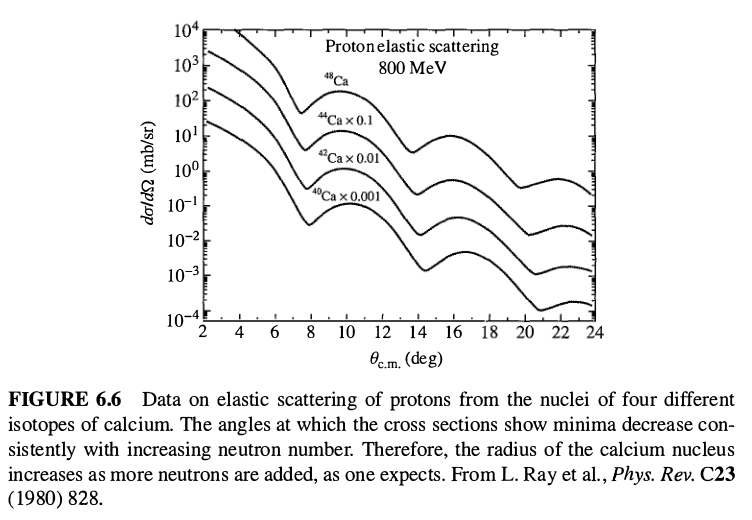
\includegraphics[width=0.7\linewidth]{fig6-6.png}
\end{figure}

\begin{tcolorbox}[breakable]
	For a square well, the scattering amplitude obtained by using the first-order Born approximation is given by Eq (6.3.7):
	\begin{align*}
		f^{(1)}(\theta) & = -\frac{2m}{\hbar^2} \frac{V_0a^3}{(qa)^2} \left[ \frac{\sin qa}{qa} - \cos qa \right]
	\end{align*}
	The first three zeros of this function can be solved numerically, which are: 4.49341, 7.72525, 10.9041
	\begin{figure}[H]
		\centering
		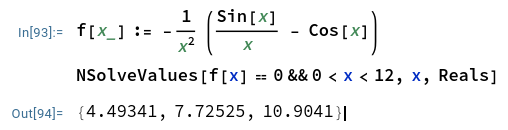
\includegraphics[width=0.5\linewidth]{figMathematicaBorn.png}
	\end{figure}

	For $^40\Ca$, The three minimas are at $\theta = 7.95^\circ, 14.2^\circ, 20.4^\circ$. For $\SI{800}{MeV}$ energy: $\hbar^2k^2/2m = \SI{800}{MeV} \iff k = \SI{4.32}{(/fm)}$. The corresponding scattering radius are:
	\begin{align*}
		q & = 2k\sin\frac{\theta}{2}                       & \iff q & = (1.20, 2.12, 3.08) \text{1/fm} \\
		a & = (4.49/1.20, 7.73/2.12, 10.90/3.08) \text{fm} & \iff a & = 3.74, 3.64, 3.54 \text{fm}
	\end{align*}

	Comparing with the empiricial value $a_{empirical} = 1.4A^{1/3} = 4.79\text{fm}$, we see that the first-order Born approximation is not a good approximation. Nevertheless, it is still useful to explain the scattering phenomenon.
\end{tcolorbox}
\end{section}

\begin{section}{Sakurai 6.5}
A spinless particle is scattered by a weak Yukawa potential
\begin{align*}
	V = \frac{V_0 e^{-\mu r}}{\mu r}
\end{align*}
where $\mu > 0$ but $V_0$ can be positive or negative. It was shown in the text that the first-order Born amplitude is given by:
\begin{align*}
	f^{(1)}(\theta) = -\frac{2m}{\hbar^2} \frac{V_0}{\mu} \left[ \frac{1}{2k^2 (1-\cos\theta) + \mu^2}\right]
\end{align*}
\begin{enumerate}
	\item Using $f^{(1)}(\theta)$ and assuming $|\delta_l| \ll 1$, obtain an expression for $\delta_l$ in terms of a Legendre function of the second kind,
	\begin{align*}
		Q_l(\zeta) = \frac{1}{2} \int_{-1}^{1} \frac{P_l(\zeta')}{\zeta - \zeta'} d\zeta'
	\end{align*}

	\begin{tcolorbox}[breakable]
		First we can begin with Eq.(6.4.40) define $x \equiv \cos\theta$ and integrate both sides to get the orthogonality condition:
		\begin{align*}
			f(x)                         & = \frac{1}{k} \sum_{l=0} (2l+1) e^{i\delta l} \sin\delta_l P_l(x)                               \\
			\int_{-1}^{1} f(x) P_l(x) dx & = \frac{1}{k} \sum_{l'=0} (2l'+1) e^{i\delta l'} \int_{-1}^{1} \sin\delta_l P_l(x) P_{l'}(x) dx \\
			                             & = \frac{1}{k} \sum_{l'=0} (2l'+1) e^{i\delta l'} \frac{2}{2l'+1} \delta_{ll'}                   \\
			                             & = \frac{2}{k}  e^{i\delta l} \sin\delta_l                                                       \\
			\int_{-1}^{1} f(x) P_l(x) dx & \approx \frac{2}{k} \delta_l
		\end{align*}

		On the other hand, we can substitute from the given expression of $f^{(1)}(\theta)$:
		\begin{align*}
			\frac{2}{k} \delta_l & = -\frac{2m}{\hbar^2} \frac{V_0}{\mu} \int_{-1}^{1}  \frac{P_l(x)}{2k^2 (1-\cos\theta) + \mu^2} dx      \\
			                     & = -\frac{2m}{\hbar^2 k^2} \frac{V_0}{\mu} \frac{1}{2} \int_{-1}^{1}  \frac{P_l(x)}{1-x + \mu^2/2k^2} dx \\
			\frac{2}{k} \delta_l & = -\frac{V_0}{E\mu} Q_l(\alpha)                                                                         \\
			\delta_l             & = -\frac{k}{2\mu} \frac{V_0}{E} Q_l(\alpha)
		\end{align*}
		where $E \equiv \hbar^2k^2/2m$ and $\alpha \equiv 1 + \mu^2/2k^2$
	\end{tcolorbox}

	\newpage
	\item Use the expansion formula to prove each assertion.
	\begin{enumerate}
		\item $\delta_l$ is negative (positive) when the potential is repulsive (attractive)
		\item When the de Broglie wavelength is much longer than the range of the potential, $\delta_l$ is proportional to $k^{2l+1}$. Find the proportionality constant.
	\end{enumerate}
	\begin{tcolorbox}[breakable]
		For the first assertion: we can see it clearly that $\delta_l \propto -V_0$. When $V_0 > 0$, the potential is repulsive, and $\delta_l < 0$. When $V_0 < 0$, the potential is attractive, and $\delta_l > 0$.

		For the second assertion: If $k \ll \mu \to \mu/k \gg 1$. Then $\alpha \approx \mu^2/2k^2 \gg 1$. We can use the expansion formula of $Q_l(\alpha)$:
		\begin{align*}
			\delta_l & = -\frac{k}{2\mu} \frac{V_0}{E} Q_l(\alpha)                                            \\
			         & = -\frac{1}{2\mu} \frac{V_0}{E} \frac{l!}{(2l+1)!}\frac{k}{\alpha^{l+1}}               \\
			         & = -\frac{1}{2\mu} \frac{V_0}{E} \frac{l!}{(2l+1)!} \frac{2^{l+1}}{\mu^{2l+2}} k^{2l+3} \\
			         & = -\frac{2^l l!}{(2l+1)!} \frac{2mV_0}{\hbar^2 \mu^{2l+2}} \frac{k^{2l+3}}{k^2}        \\
			         & = -\frac{2^{l+1} l!}{(2l+1)!} \frac{m V_0}{\hbar^2 \mu^{2l+3}} k^{2l+1}                \\
		\end{align*}
	\end{tcolorbox}
\end{enumerate}
\end{section}

\newpage
\begin{section}{Problem 6.7}
Consider the scattering of a particle by an impenetrable sphere
\begin{align*}
	V(r) = \begin{cases}
		       0      & r \geq a \\
		       \infty & r < a
	       \end{cases}
\end{align*}
\begin{enumerate}
	\item Derive an expression for the s-wave (l=0) phase shift.
	\item What is the total cross section $\sigma = \int(d\sigma/d\Omega) d\Omega$ in the extreme low-energy limit $k \to 0$? Compare your anser with the geometric cross section $\pi a^2$.
\end{enumerate}

\begin{tcolorbox}[breakable]
	The condition implies that all wave function must vanish at $r > a$. The wavefunction at $r > a$ is given by Eq.(6.4.52):
	\begin{align*}
		A_l(r) & = e^{i\delta_l} \left[ \cos\delta_l j_l(ka) - \sin\delta_l n_l(ka)\right]
	\end{align*}
	The condition $A_l(r) = 0$ gives:
	\begin{align*}
		\tan \delta_l & = \frac{j_l(ka)}{n_l(ka)}
	\end{align*}
	For s-wave ($l=0$), we have:
	\begin{align*}
		\tan \delta_0 & = \frac{j_0(ka)}{n_0(ka)} = \frac{\sin(ka)/ka}{-\cos(ka)/ka} = -\tan(ka)
	\end{align*}
	Therefore $\delta_0 \propto -ka$:
	\begin{align*}
		A_{l=0}(r) & = e^{i\delta_0} \left( \frac{\sin(kr)}{kr} \cos(kr) + \frac{\cos(kr)}{kr}\sin(kr)\right) \\
		           & \propto \frac{e^{i\delta_0}}{kr} \left( \sin(kr + \delta_0) \right)                      \\
		           & \propto \frac{e^{i\delta_0}}{kr} \left( \sin(kr - ka) \right)
	\end{align*}

	In the extreme low-energy limit. For $k \ll 1$:
	\begin{align*}
		\frac{d\sigma}{d\Omega} = \frac{\sin^2 \delta_0}{k^2} \approx a^2
	\end{align*}
	The total cross section is:
	\begin{align*}
		\sigma = \int \frac{d\sigma}{d\Omega} d\Omega = 4\pi a^2
	\end{align*}
	which is exactly four times the geometric cross section.
\end{tcolorbox}
\end{section}
\end{document}
